\documentclass[11pt,letterpaper]{article}

\usepackage[utf8]{inputenc}
\usepackage[T1]{fontenc}
\usepackage[spanish,es-tabla]{babel}
\usepackage{lmodern}
\usepackage[margin=2.5cm]{geometry}
\usepackage{graphicx}
\usepackage{booktabs}
\usepackage{tabularx}
\usepackage{xcolor}
\usepackage{listings}
\usepackage{float}
\usepackage{caption}
\usepackage[hidelinks]{hyperref}

\definecolor{verde}{RGB}{46,125,50}
\definecolor{fondo}{RGB}{246,246,246}

\newcommand{\ok}{\textcolor{verde}{\textbf{Pasa}}}

% Bloques de código y de salida de consola
\lstset{
  basicstyle=\ttfamily\footnotesize,
  backgroundcolor=\color{fondo},
  frame=single, rulecolor=\color{gray!40},
  breaklines=true, columns=fullflexible, keepspaces=true,
  showstringspaces=false,
  literate={á}{{\'a}}1 {é}{{\'e}}1 {í}{{\'i}}1 {ó}{{\'o}}1 {ú}{{\'u}}1
           {Á}{{\'A}}1 {É}{{\'E}}1 {Í}{{\'I}}1 {Ó}{{\'O}}1 {Ú}{{\'U}}1
           {ñ}{{\~n}}1 {Ñ}{{\~N}}1 {«}{{\guillemotleft}}1 {»}{{\guillemotright}}1
}
\lstdefinestyle{java}{language=Java, keywordstyle=\color{purple!70!black}\bfseries,
  commentstyle=\color{verde}, stringstyle=\color{blue!70!black},
  morekeywords={record}, emph={[2]Stateless,Singleton,Local,Inject,ApplicationException},
  emphstyle={[2]\color{orange!70!black}}}

% Captura de Postman
\newcommand{\captura}[2]{%
  \begin{figure}[H]
    \centering
    \includegraphics[width=0.92\linewidth]{capturas/#1}
    \caption{#2}
  \end{figure}}

\title{\textbf{Taller No.~2 Jakarta EE + Tier de Negocio}\\[4pt]
  \large Diseño de la arquitectura y evidencias de funcionamiento\\
  Módulo de gestión de solicitudes de recursos}
\author{Nombre del estudiante\\
  \small Arquitectura de Software -- Departamento de Ingeniería de Sistemas\\
  \small Pontificia Universidad Javeriana}
\date{2026-30}

\begin{document}
\sloppy
\maketitle

\begin{abstract}
\noindent Se implementó el tier de negocio de un módulo que administra las solicitudes de
recursos durante emergencias. Las reglas de negocio viven en un EJB de sesión
\texttt{@Stateless}, que solo conoce una interfaz de repositorio; el tier de datos la
implementa con una colección en memoria. El documento presenta la arquitectura, explica cómo
se desacopló el negocio de la persistencia y muestra las evidencias: 13 pruebas unitarias
del EJB sin servidor y 13 peticiones REST con 24 aserciones sobre Payara~7. Todas pasan.
\end{abstract}

\tableofcontents
\newpage

% =====================================================================
\section{Arquitectura propuesta}

La solución es una aplicación Jakarta EE~11 empaquetada como un único WAR
(\texttt{negocio-jee.war}) y desplegada en Payara~7. Internamente se organiza en tres capas
lógicas más un modelo de dominio compartido:

\begin{itemize}
  \item \textbf{Presentación (REST).} Endpoints JAX-RS delgados que solo traducen HTTP/JSON a
        llamadas al negocio. Existen para evidenciar el funcionamiento; no contienen reglas.
  \item \textbf{Negocio (EJB).} El EJB de sesión sin estado \texttt{GestionSolicitudesBean}
        encapsula todas las reglas. Se expone por la interfaz local \texttt{GestionSolicitudes}.
  \item \textbf{Datos (en memoria).} \texttt{SolicitudRepositoryMemoria}, un EJB
        \texttt{@Singleton} que guarda las solicitudes en un \texttt{ConcurrentHashMap}.
\end{itemize}

La regla que gobierna el diseño es que \textbf{las dependencias siempre apuntan hacia el
tier de negocio}: la presentación depende del negocio y los datos dependen del negocio; el
negocio no depende de ninguno de los dos.

\begin{figure}[H]
  \centering
  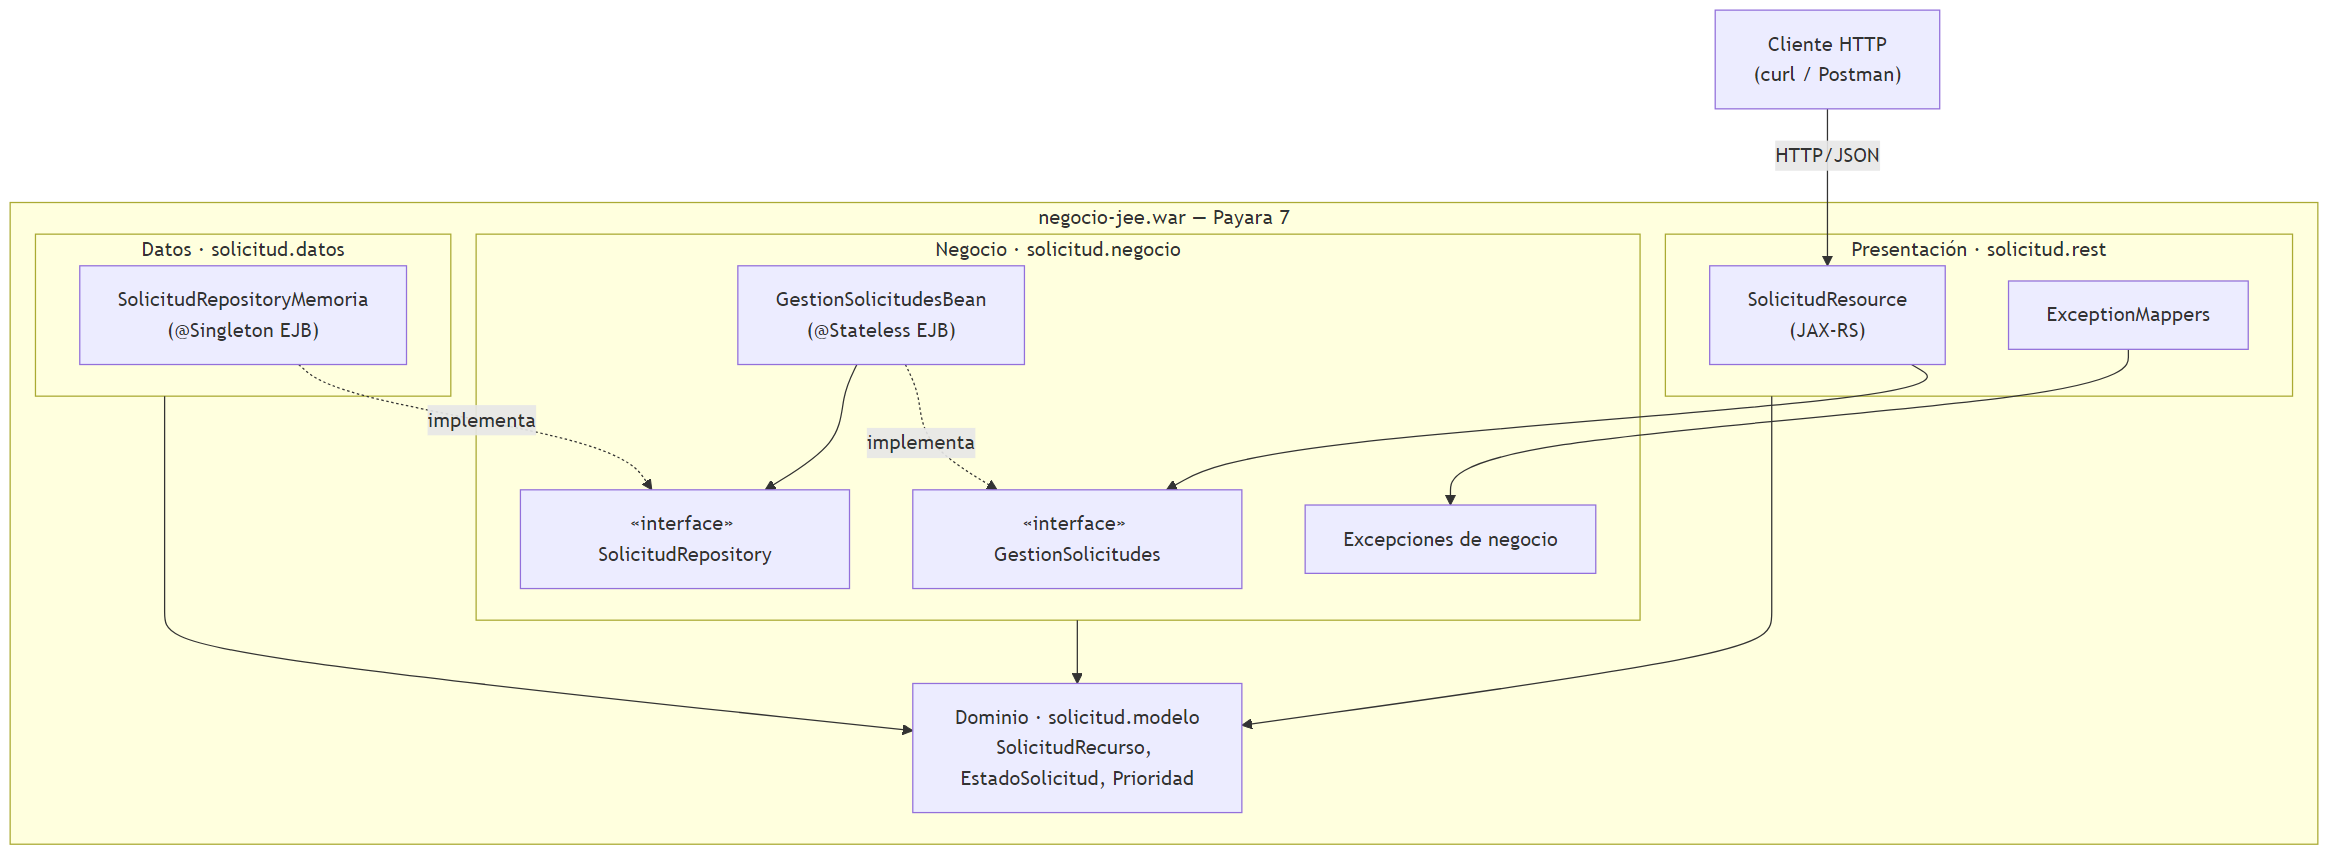
\includegraphics[width=\linewidth]{diagramas/02-componentes.png}
  \caption{Capas y colaboración entre componentes.}
\end{figure}

\begin{table}[H]
\centering\small
\caption{Paquetes de \texttt{edu.javeriana.negocio.jakarta} y su tier.}
\begin{tabularx}{\linewidth}{l >{\raggedright\arraybackslash}X l}
\toprule
\textbf{Paquete} & \textbf{Contenido} & \textbf{Tier} \\
\midrule
\texttt{solicitud.rest}      & \texttt{SolicitudResource} y tres \texttt{ExceptionMapper} & Presentación \\
\texttt{solicitud.rest.dto}  & \texttt{SolicitudEntrada}, \texttt{SolicitudSalida}, \texttt{ErrorSalida} & Presentación \\
\texttt{solicitud.negocio}   & \texttt{GestionSolicitudes} (\texttt{@Local}), \texttt{GestionSolicitudesBean}
                               (\texttt{@Stateless}), \texttt{SolicitudRepository}, excepciones & Negocio \\
\texttt{solicitud.modelo}    & \texttt{SolicitudRecurso}, \texttt{EstadoSolicitud}, \texttt{Prioridad} & Dominio \\
\texttt{solicitud.datos}     & \texttt{SolicitudRepositoryMemoria} (\texttt{@Singleton}) & Datos \\
\texttt{hello}               & \texttt{HelloApplication}: activa JAX-RS en \texttt{/rest} & Configuración \\
\bottomrule
\end{tabularx}
\end{table}

\begin{figure}[H]
  \centering
  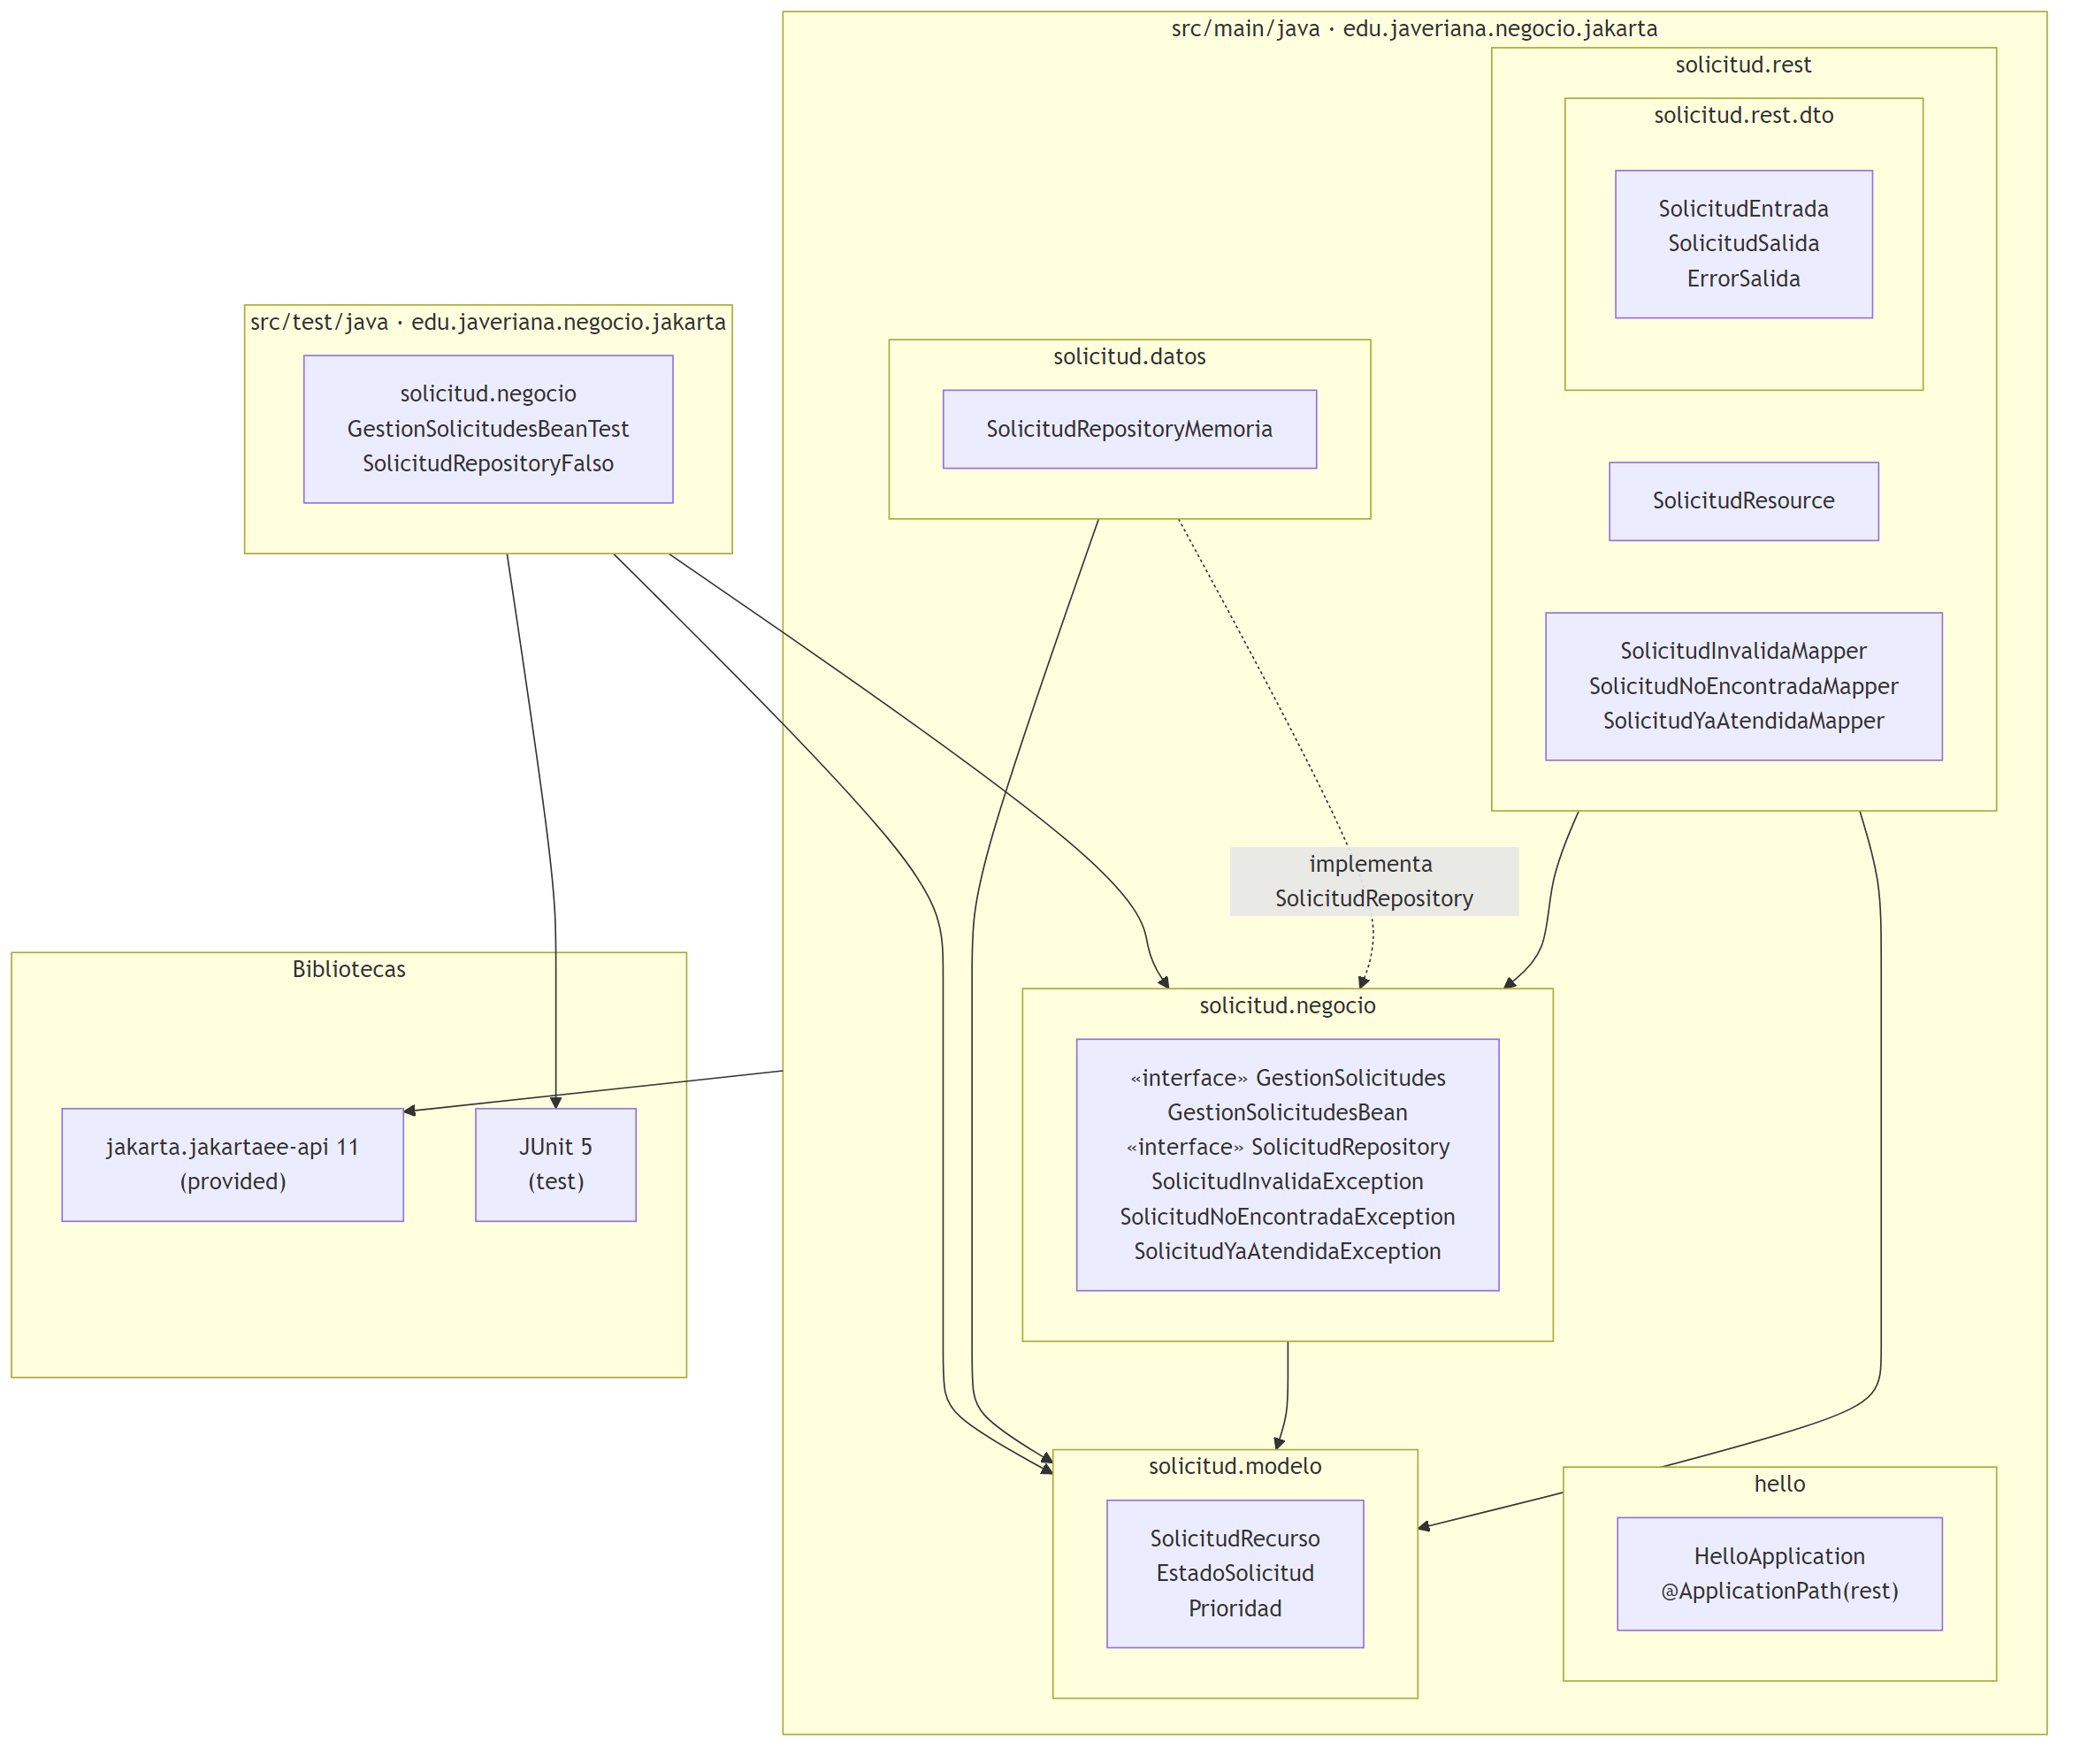
\includegraphics[width=0.95\linewidth]{diagramas/01-paquetes.png}
  \caption{Diagrama de paquetes. Las flechas punteadas indican que un paquete implementa una
  interfaz definida en otro.}
\end{figure}

\subsection{Contrato REST}

Ruta base: \texttt{http://localhost:8080/negocio-jee/rest}. Los DTO son el contrato JSON y
viven solo en la capa REST: \texttt{SolicitudEntrada} no tiene \texttt{id} ni
\texttt{estado}, de modo que el cliente no puede fijarlos.

\begin{table}[H]
\centering\small
\caption{Operaciones expuestas.}
\begin{tabularx}{\linewidth}{>{\raggedright\arraybackslash}X l l}
\toprule
\textbf{Operación} & \textbf{Método y ruta} & \textbf{Respuestas} \\
\midrule
Registrar solicitud      & \texttt{POST /solicitudes}             & 201 · 400 \\
Consultar todas          & \texttt{GET /solicitudes}              & 200 \\
Buscar por identificador & \texttt{GET /solicitudes/\{id\}}       & 200 · 404 \\
Consultar pendientes     & \texttt{GET /solicitudes/pendientes}   & 200 \\
Atender solicitud        & \texttt{PUT /solicitudes/\{id\}/atender} & 200 · 404 · 409 \\
\bottomrule
\end{tabularx}
\end{table}

\subsection{Máquina de estados}

Una solicitud tiene una única transición válida, de \texttt{PENDIENTE} a \texttt{ATENDIDA}.
La controla el EJB: es el único componente que asigna el estado.

\begin{figure}[H]
  \centering
  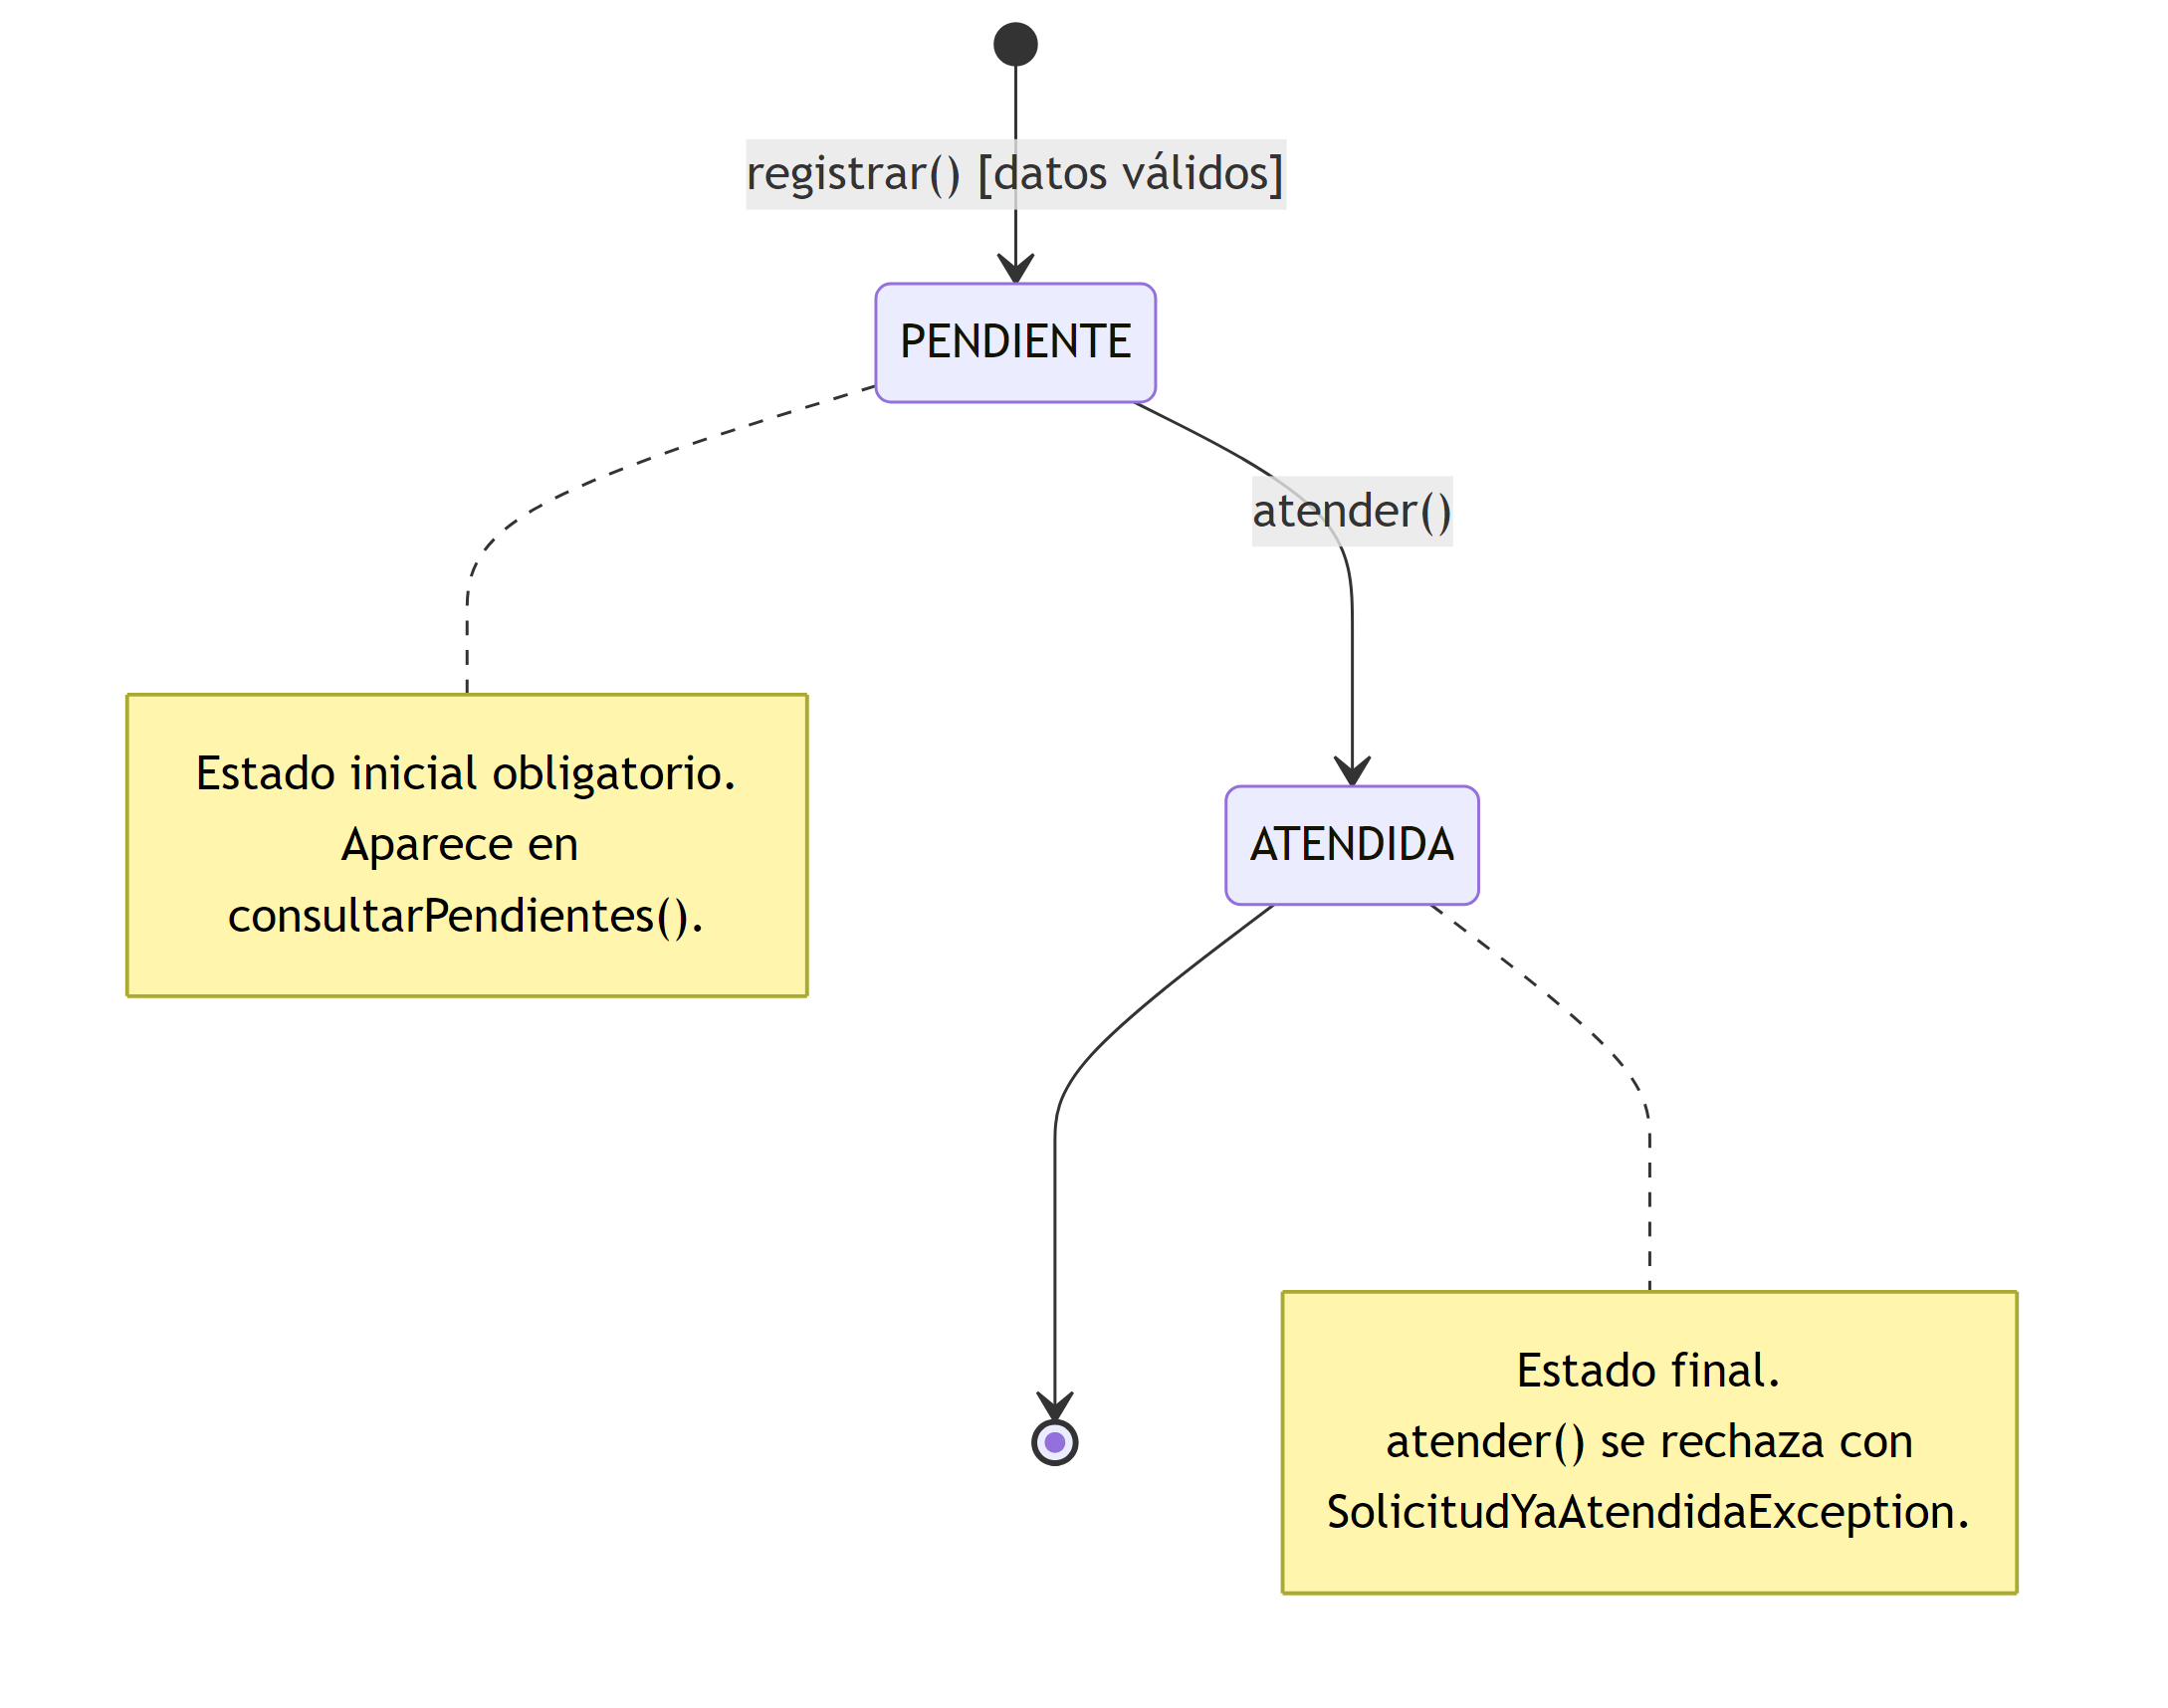
\includegraphics[width=0.6\linewidth]{diagramas/04-estados.png}
  \caption{Máquina de estados de la solicitud.}
\end{figure}

% =====================================================================
\section{Desacoplamiento entre el tier de negocio y el tier de datos}

El EJB de negocio no sabe cómo ni dónde se guardan las solicitudes. Esto se logra con cinco
decisiones:

\begin{enumerate}
  \item \textbf{Inversión de dependencias.} La interfaz \texttt{SolicitudRepository}
        pertenece al paquete \emph{de negocio} y expresa lo que el negocio necesita de la
        persistencia (guardar, actualizar, buscar, listar). El tier de datos la implementa.
        Por eso \texttt{solicitud.negocio} no importa ninguna clase de \texttt{solicitud.datos}:
        la dependencia va de datos hacia negocio y no al revés.
  \item \textbf{Inyección por el contenedor.} El EJB declara
        \texttt{@Inject SolicitudRepository} y el contenedor le entrega la implementación
        disponible. Nunca hace \texttt{new SolicitudRepositoryMemoria()}.
  \item \textbf{Sustituibilidad.} Para pasar a una base de datos basta con escribir otra
        clase, por ejemplo \texttt{SolicitudRepositoryJpa}, que implemente la misma interfaz.
        Ni el EJB ni la capa REST cambian.
  \item \textbf{Repositorio sin reglas.} \texttt{SolicitudRepositoryMemoria} solo almacena,
        recupera y genera el identificador. No valida ni cambia estados.
  \item \textbf{Negocio que se prueba sin servidor.} Como el EJB solo depende de una interfaz, las
        pruebas JUnit lo crean con \texttt{new} y un repositorio falso. Que todas las reglas
        se cumplan así es la evidencia de que el negocio no está atado a la persistencia.
\end{enumerate}

\begin{lstlisting}[style=java]
// solicitud.negocio: la interfaz la define el negocio, no el tier de datos
public interface SolicitudRepository {
    SolicitudRecurso guardar(SolicitudRecurso solicitud);
    SolicitudRecurso actualizar(SolicitudRecurso solicitud);
    Optional<SolicitudRecurso> buscarPorId(long id);
    List<SolicitudRecurso> listarTodas();
}

// solicitud.negocio: el EJB solo conoce la interfaz
@Stateless
public class GestionSolicitudesBean implements GestionSolicitudes {
    @Inject
    private SolicitudRepository repositorio;
    ...
}

// solicitud.datos: el tier de datos implementa la interfaz del negocio
@Singleton
public class SolicitudRepositoryMemoria implements SolicitudRepository { ... }
\end{lstlisting}

El mismo principio se aplica hacia arriba: la capa REST depende de la interfaz
\texttt{GestionSolicitudes}, no de la clase del EJB.

\begin{figure}[H]
  \centering
  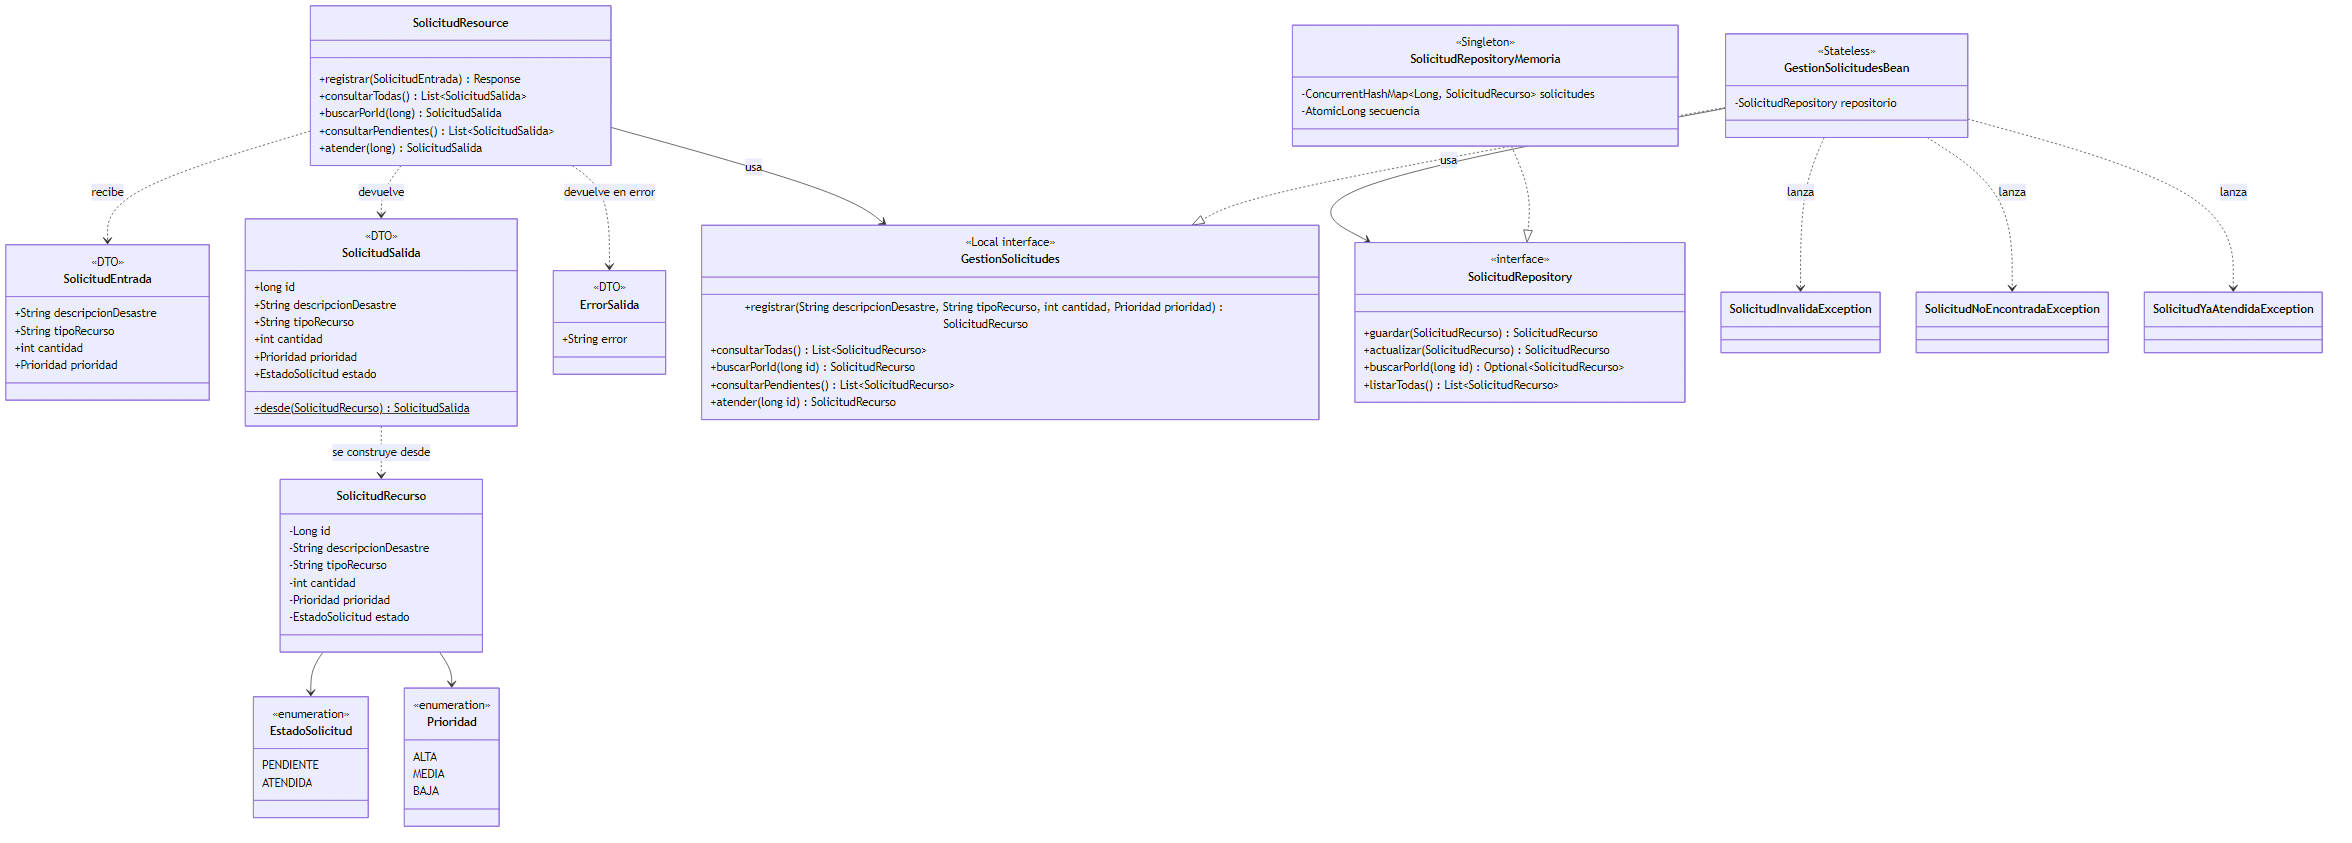
\includegraphics[width=\linewidth]{diagramas/03-clases.png}
  \caption{Diagrama de clases.}
\end{figure}

\subsection{Decisiones y supuestos}

\begin{itemize}
  \item \textbf{\texttt{@Stateless} para el negocio:} las operaciones no guardan estado
        conversacional, así que el contenedor puede reutilizar instancias.
  \item \textbf{\texttt{@Singleton} para el almacén:} la colección debe ser única y compartida
        por todas las instancias del EJB de negocio; además se usan \texttt{ConcurrentHashMap}
        y \texttt{AtomicLong}.
  \item \textbf{Interfaz \texttt{@Local}:} el único cliente (la capa REST) está en la misma
        JVM; no se necesita una interfaz \texttt{@Remote}.
  \item \textbf{Excepciones de aplicación:} las excepciones de negocio llevan
        \texttt{@ApplicationException}, así el contenedor no las envuelve en
        \texttt{EJBException} y la capa REST las traduce a 400, 404 o 409.
  \item \textbf{Prioridad:} el enunciado no define sus valores; se modela como enumerado
        \texttt{ALTA}, \texttt{MEDIA}, \texttt{BAJA} y se trata como dato obligatorio.
  \item \textbf{Sin persistencia duradera:} los datos se pierden al reiniciar el servidor,
        lo que el enunciado admite al pedir una colección en memoria.
\end{itemize}

% =====================================================================
\section{Cobertura de las reglas de negocio}

Todas las validaciones se ejecutan en \texttt{GestionSolicitudesBean}. La
Tabla~\ref{tab:reglas} relaciona cada regla del enunciado con la prueba unitaria y la
petición de Postman que la verifican.

\begin{table}[H]
\centering\small
\caption{Reglas de negocio y pruebas que las verifican.}
\label{tab:reglas}
\begin{tabularx}{\linewidth}{>{\raggedright\arraybackslash}X l l c}
\toprule
\textbf{Regla} & \textbf{Prueba JUnit} & \textbf{Postman} & \textbf{HTTP} \\
\midrule
La cantidad debe ser mayor que cero & \texttt{rechazarCantidadCeroONegativa} & 03 & 400 \\
La descripción del desastre es obligatoria & \texttt{rechazarSinDescripcion} & 04 & 400 \\
El tipo de recurso es obligatorio & \texttt{rechazarSinTipoRecurso} & 05 & 400 \\
La prioridad es obligatoria (supuesto) & \texttt{rechazarSinPrioridad} & 06 & 400 \\
Toda solicitud nueva inicia en \texttt{PENDIENTE} & \texttt{registrarSolicitudValida} & 01 & 201 \\
No se atiende una solicitud inexistente & \texttt{atenderInexistente} & 12 & 404 \\
No se atiende dos veces la misma solicitud & \texttt{atenderDosVeces} & 11 & 409 \\
Las validaciones ocurren en el negocio & todas (sin servidor ni REST) & --- & --- \\
\bottomrule
\end{tabularx}
\end{table}

La última regla queda demostrada por la forma de las pruebas unitarias: crean el EJB con
\texttt{new} y un repositorio falso, sin capa REST ni servidor, y aun así todas las
validaciones se cumplen.

% =====================================================================
\section{Pruebas unitarias del EJB}

\subsection{Cómo se prueba el EJB sin servidor}

\begin{lstlisting}[style=java]
class GestionSolicitudesBeanTest {

    private GestionSolicitudesBean gestion;

    @BeforeEach
    void prepararEjb() {
        gestion = new GestionSolicitudesBean(new SolicitudRepositoryFalso());
    }

    @Test
    @DisplayName("No se puede atender dos veces la misma solicitud")
    void atenderDosVeces() {
        SolicitudRecurso creada = registrarValida();
        gestion.atender(creada.getId());

        assertThrows(SolicitudYaAtendidaException.class,
                     () -> gestion.atender(creada.getId()));
    }
}
\end{lstlisting}

\subsection{Resultados}

\begin{table}[H]
\centering\small
\caption{Pruebas unitarias de \texttt{GestionSolicitudesBean}.}
\begin{tabularx}{\linewidth}{r l >{\raggedright\arraybackslash}X c}
\toprule
\textbf{\#} & \textbf{Método} & \textbf{Qué verifica} & \textbf{Resultado} \\
\midrule
1  & \texttt{registrarSolicitudValida}      & Se registra con id y en estado \texttt{PENDIENTE} & \ok \\
2  & \texttt{rechazarCantidadCeroONegativa} & Cantidad 0 y $-5$ se rechazan & \ok \\
3  & \texttt{rechazarSinDescripcion}        & Descripción nula o en blanco se rechaza & \ok \\
4  & \texttt{rechazarSinTipoRecurso}        & Tipo de recurso vacío se rechaza & \ok \\
5  & \texttt{rechazarSinPrioridad}          & Prioridad nula se rechaza & \ok \\
6  & \texttt{solicitudInvalidaNoSeGuarda}   & Una solicitud rechazada no queda guardada & \ok \\
7  & \texttt{consultarTodas}                & Devuelve todas las registradas & \ok \\
8  & \texttt{buscarPorId}                   & Devuelve la solicitud pedida & \ok \\
9  & \texttt{buscarIdInexistente}           & Lanza \texttt{SolicitudNoEncontradaException} & \ok \\
10 & \texttt{consultarPendientes}           & Excluye las atendidas & \ok \\
11 & \texttt{atenderPendiente}              & Pasa a \texttt{ATENDIDA} y queda guardado & \ok \\
12 & \texttt{atenderInexistente}            & Lanza \texttt{SolicitudNoEncontradaException} & \ok \\
13 & \texttt{atenderDosVeces}               & Lanza \texttt{SolicitudYaAtendidaException} & \ok \\
\bottomrule
\end{tabularx}
\end{table}

Salida de \texttt{mvn clean package} (extracto; la salida completa está en
\texttt{evidencias/maven-build.txt}):

\begin{lstlisting}
[INFO] -------------------------------------------------------
[INFO]  T E S T S
[INFO] -------------------------------------------------------
[INFO] Running edu.javeriana.negocio.jakarta.solicitud.negocio.GestionSolicitudesBeanTest
[INFO] Tests run: 13, Failures: 0, Errors: 0, Skipped: 0
[INFO]
[INFO] Results:
[INFO]
[INFO] Tests run: 13, Failures: 0, Errors: 0, Skipped: 0
[INFO]
[INFO] --- war:3.5.1:war (default-war) @ negocio-jee ---
[INFO] Building war: target/negocio-jee.war
[INFO] BUILD SUCCESS
\end{lstlisting}

% =====================================================================
\section{Pruebas sobre Payara con Postman}

La colección \texttt{postman/negocio-jee.postman\_collection.json} contiene 13 peticiones
que se ejecutan en orden sobre un servidor recién iniciado. Cada una tiene aserciones
automáticas que comprueban el código HTTP y el contenido de la respuesta.

\begin{table}[H]
\centering\small
\caption{Peticiones de la colección y resultado obtenido sobre Payara~7.}
\begin{tabularx}{\linewidth}{r >{\raggedright\arraybackslash}X l c c}
\toprule
\textbf{\#} & \textbf{Caso} & \textbf{Petición} & \textbf{Esperado} & \textbf{Obtenido} \\
\midrule
01 & Registrar solicitud válida      & \texttt{POST /solicitudes}             & 201 & 201 \\
02 & Registrar segunda solicitud     & \texttt{POST /solicitudes}             & 201 & 201 \\
03 & Cantidad cero                   & \texttt{POST /solicitudes}             & 400 & 400 \\
04 & Descripción vacía               & \texttt{POST /solicitudes}             & 400 & 400 \\
05 & Tipo de recurso vacío           & \texttt{POST /solicitudes}             & 400 & 400 \\
06 & Sin prioridad                   & \texttt{POST /solicitudes}             & 400 & 400 \\
07 & Consultar todas                 & \texttt{GET /solicitudes}              & 200 & 200 \\
08 & Buscar por id                   & \texttt{GET /solicitudes/1}            & 200 & 200 \\
09 & Buscar id inexistente           & \texttt{GET /solicitudes/999}          & 404 & 404 \\
10 & Atender solicitud pendiente     & \texttt{PUT /solicitudes/1/atender}    & 200 & 200 \\
11 & Atender dos veces               & \texttt{PUT /solicitudes/1/atender}    & 409 & 409 \\
12 & Atender inexistente             & \texttt{PUT /solicitudes/999/atender}  & 404 & 404 \\
13 & Consultar pendientes            & \texttt{GET /solicitudes/pendientes}   & 200 & 200 \\
\bottomrule
\end{tabularx}
\end{table}

\subsection{Registrar una solicitud}

El cliente no envía \texttt{id} ni \texttt{estado}: el repositorio asigna el identificador y
el EJB fija el estado \texttt{PENDIENTE}.

\captura{postman-01-registrar.png}{Petición 01: registro de una solicitud válida (201 Created).
Arriba el cuerpo enviado; abajo la respuesta con \texttt{id} 1 y estado \texttt{PENDIENTE}.}

\subsection{Validaciones del negocio}

Cuando el EJB rechaza los datos, lanza \texttt{SolicitudInvalidaException} y un
\texttt{ExceptionMapper} la convierte en un 400 con el mensaje de la regla. Las peticiones
03 a 06 prueban cada validación:

\begin{lstlisting}
04  descripcionDesastre: ""  ->  400 { "error": "La descripción del desastre es obligatoria" }
05  tipoRecurso: ""          ->  400 { "error": "El tipo de recurso es obligatorio" }
06  sin prioridad            ->  400 { "error": "La prioridad es obligatoria" }
\end{lstlisting}

\captura{postman-03-cantidad-cero.png}{Petición 03: solicitud rechazada por cantidad cero
(400 Bad Request).}

\subsection{Consultar}

Solo aparecen las dos solicitudes válidas: las cuatro rechazadas nunca llegaron al
repositorio. Buscar un identificador inexistente (petición 09) responde 404 con el mensaje
\emph{No existe una solicitud con id 999}.

\captura{postman-07-consultar-todas.png}{Petición 07: consulta de todas las solicitudes
(200 OK); solo están las dos registradas con datos válidos.}

\subsection{Atender una solicitud}

\captura{postman-10-atender.png}{Petición 10: la solicitud 1 pasa de \texttt{PENDIENTE} a
\texttt{ATENDIDA} (200 OK).}

\captura{postman-11-atender-dos-veces.png}{Petición 11: intento de atender de nuevo la
solicitud 1 (409 Conflict).}

Atender un identificador inexistente (petición 12) responde 404 con el mismo mensaje.

\subsection{Consultar pendientes}

La solicitud 1 ya no aparece porque fue atendida.

\captura{postman-13-pendientes.png}{Petición 13: consulta de pendientes (200 OK); solo
aparece la solicitud 2.}

\subsection{Ejecución completa de la colección}

Con el servidor reiniciado se ejecutó la colección completa en el Collection Runner de
Postman y en Newman, su ejecutor de línea de comandos (\texttt{evidencias/newman-salida.txt}):

\begin{lstlisting}
|                         |          executed |            failed |
|              iterations |                 1 |                 0 |
|                requests |                13 |                 0 |
|            test-scripts |                13 |                 0 |
|              assertions |                24 |                 0 |
\end{lstlisting}

\captura{postman-runner.png}{Collection Runner de Postman: 13 peticiones, 24 aserciones
aprobadas y 0 errores.}

% =====================================================================
\section{Conclusión}

Las 13 pruebas unitarias y las 24 aserciones de la colección de Postman pasan. Las cuatro
operaciones del enunciado (registrar, consultar todas y por identificador, atender y
consultar pendientes) funcionan sobre Payara~7, y cada regla de negocio se verifica en los
dos niveles. Como las pruebas unitarias ejecutan el EJB con un repositorio distinto del
real y sin servidor, también evidencian que el tier de negocio está desacoplado del tier
de datos y que las validaciones no dependen de la interfaz.

\section*{Cómo reproducir}

\begin{lstlisting}
mvn clean package      # compila y ejecuta las 13 pruebas JUnit
mvn cargo:run          # despliega en Payara 7 (http://localhost:8080)

# Alternativa con Docker
docker build -t negocio-jee .
docker run -p 8080:8080 negocio-jee

# Postman: Import -> postman/negocio-jee.postman_collection.json -> Run collection
# (el servidor debe estar recién iniciado)
\end{lstlisting}

\appendix
\section{Vista dinámica}

\begin{figure}[H]
  \centering
  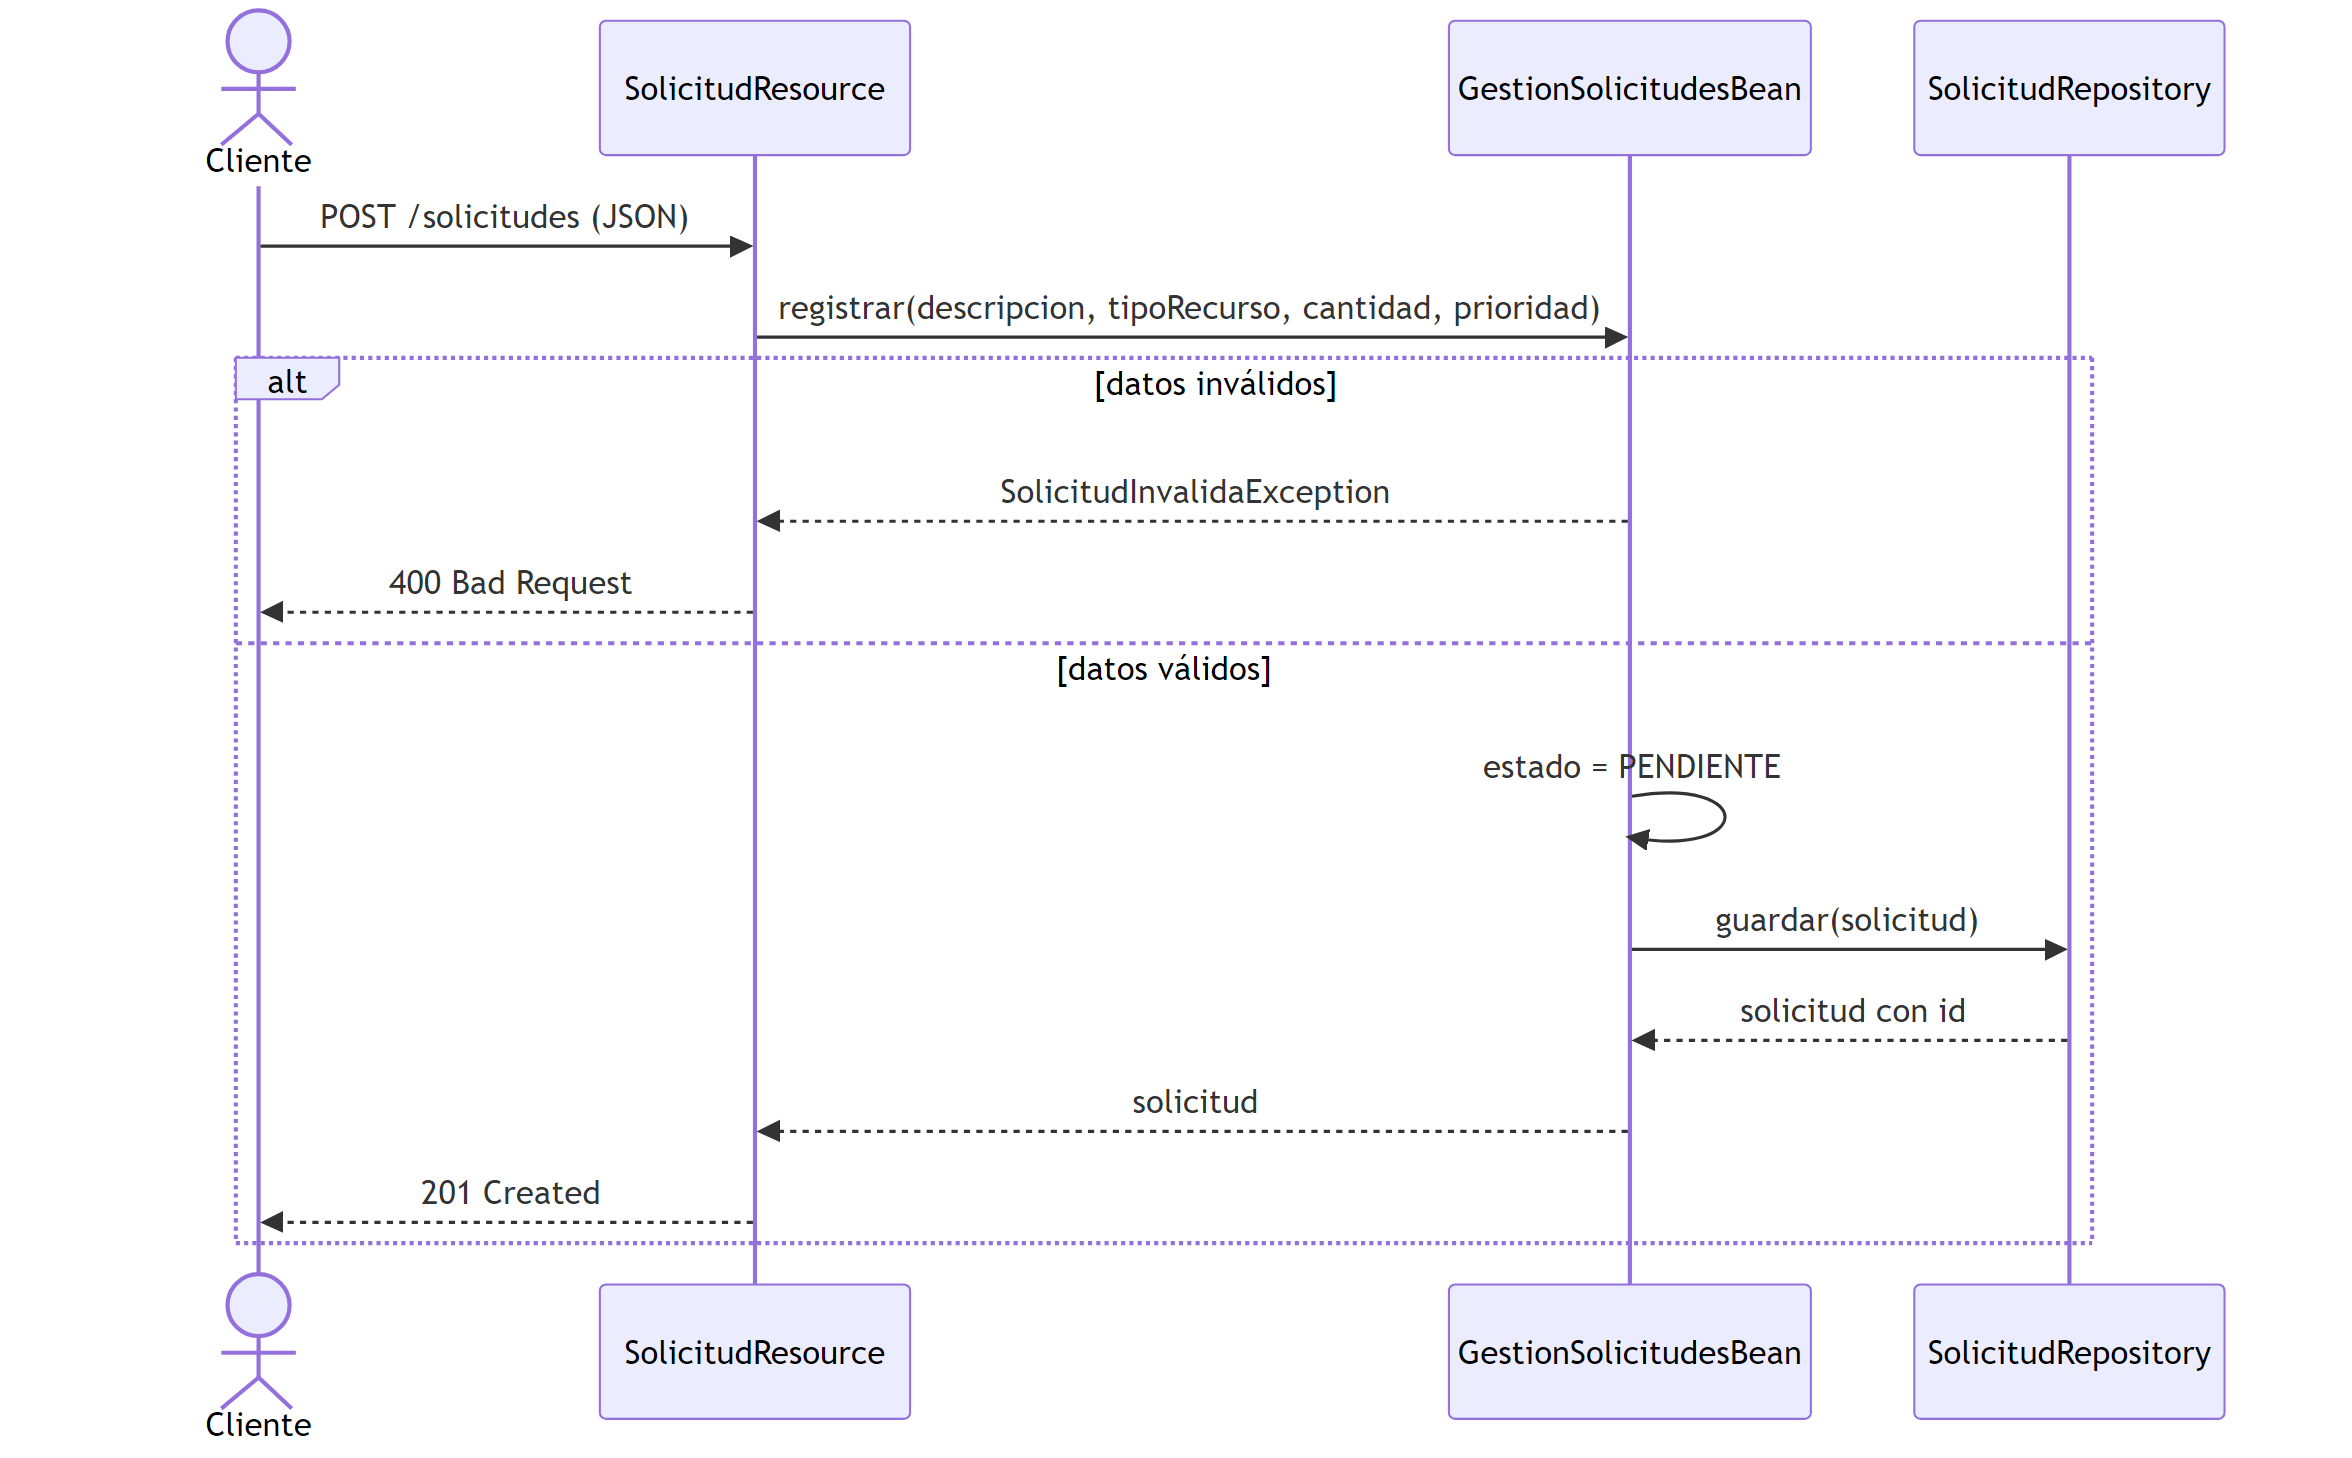
\includegraphics[width=0.8\linewidth]{diagramas/05-secuencia-registrar.png}
  \caption{Secuencia: registrar una solicitud.}
\end{figure}

\begin{figure}[H]
  \centering
  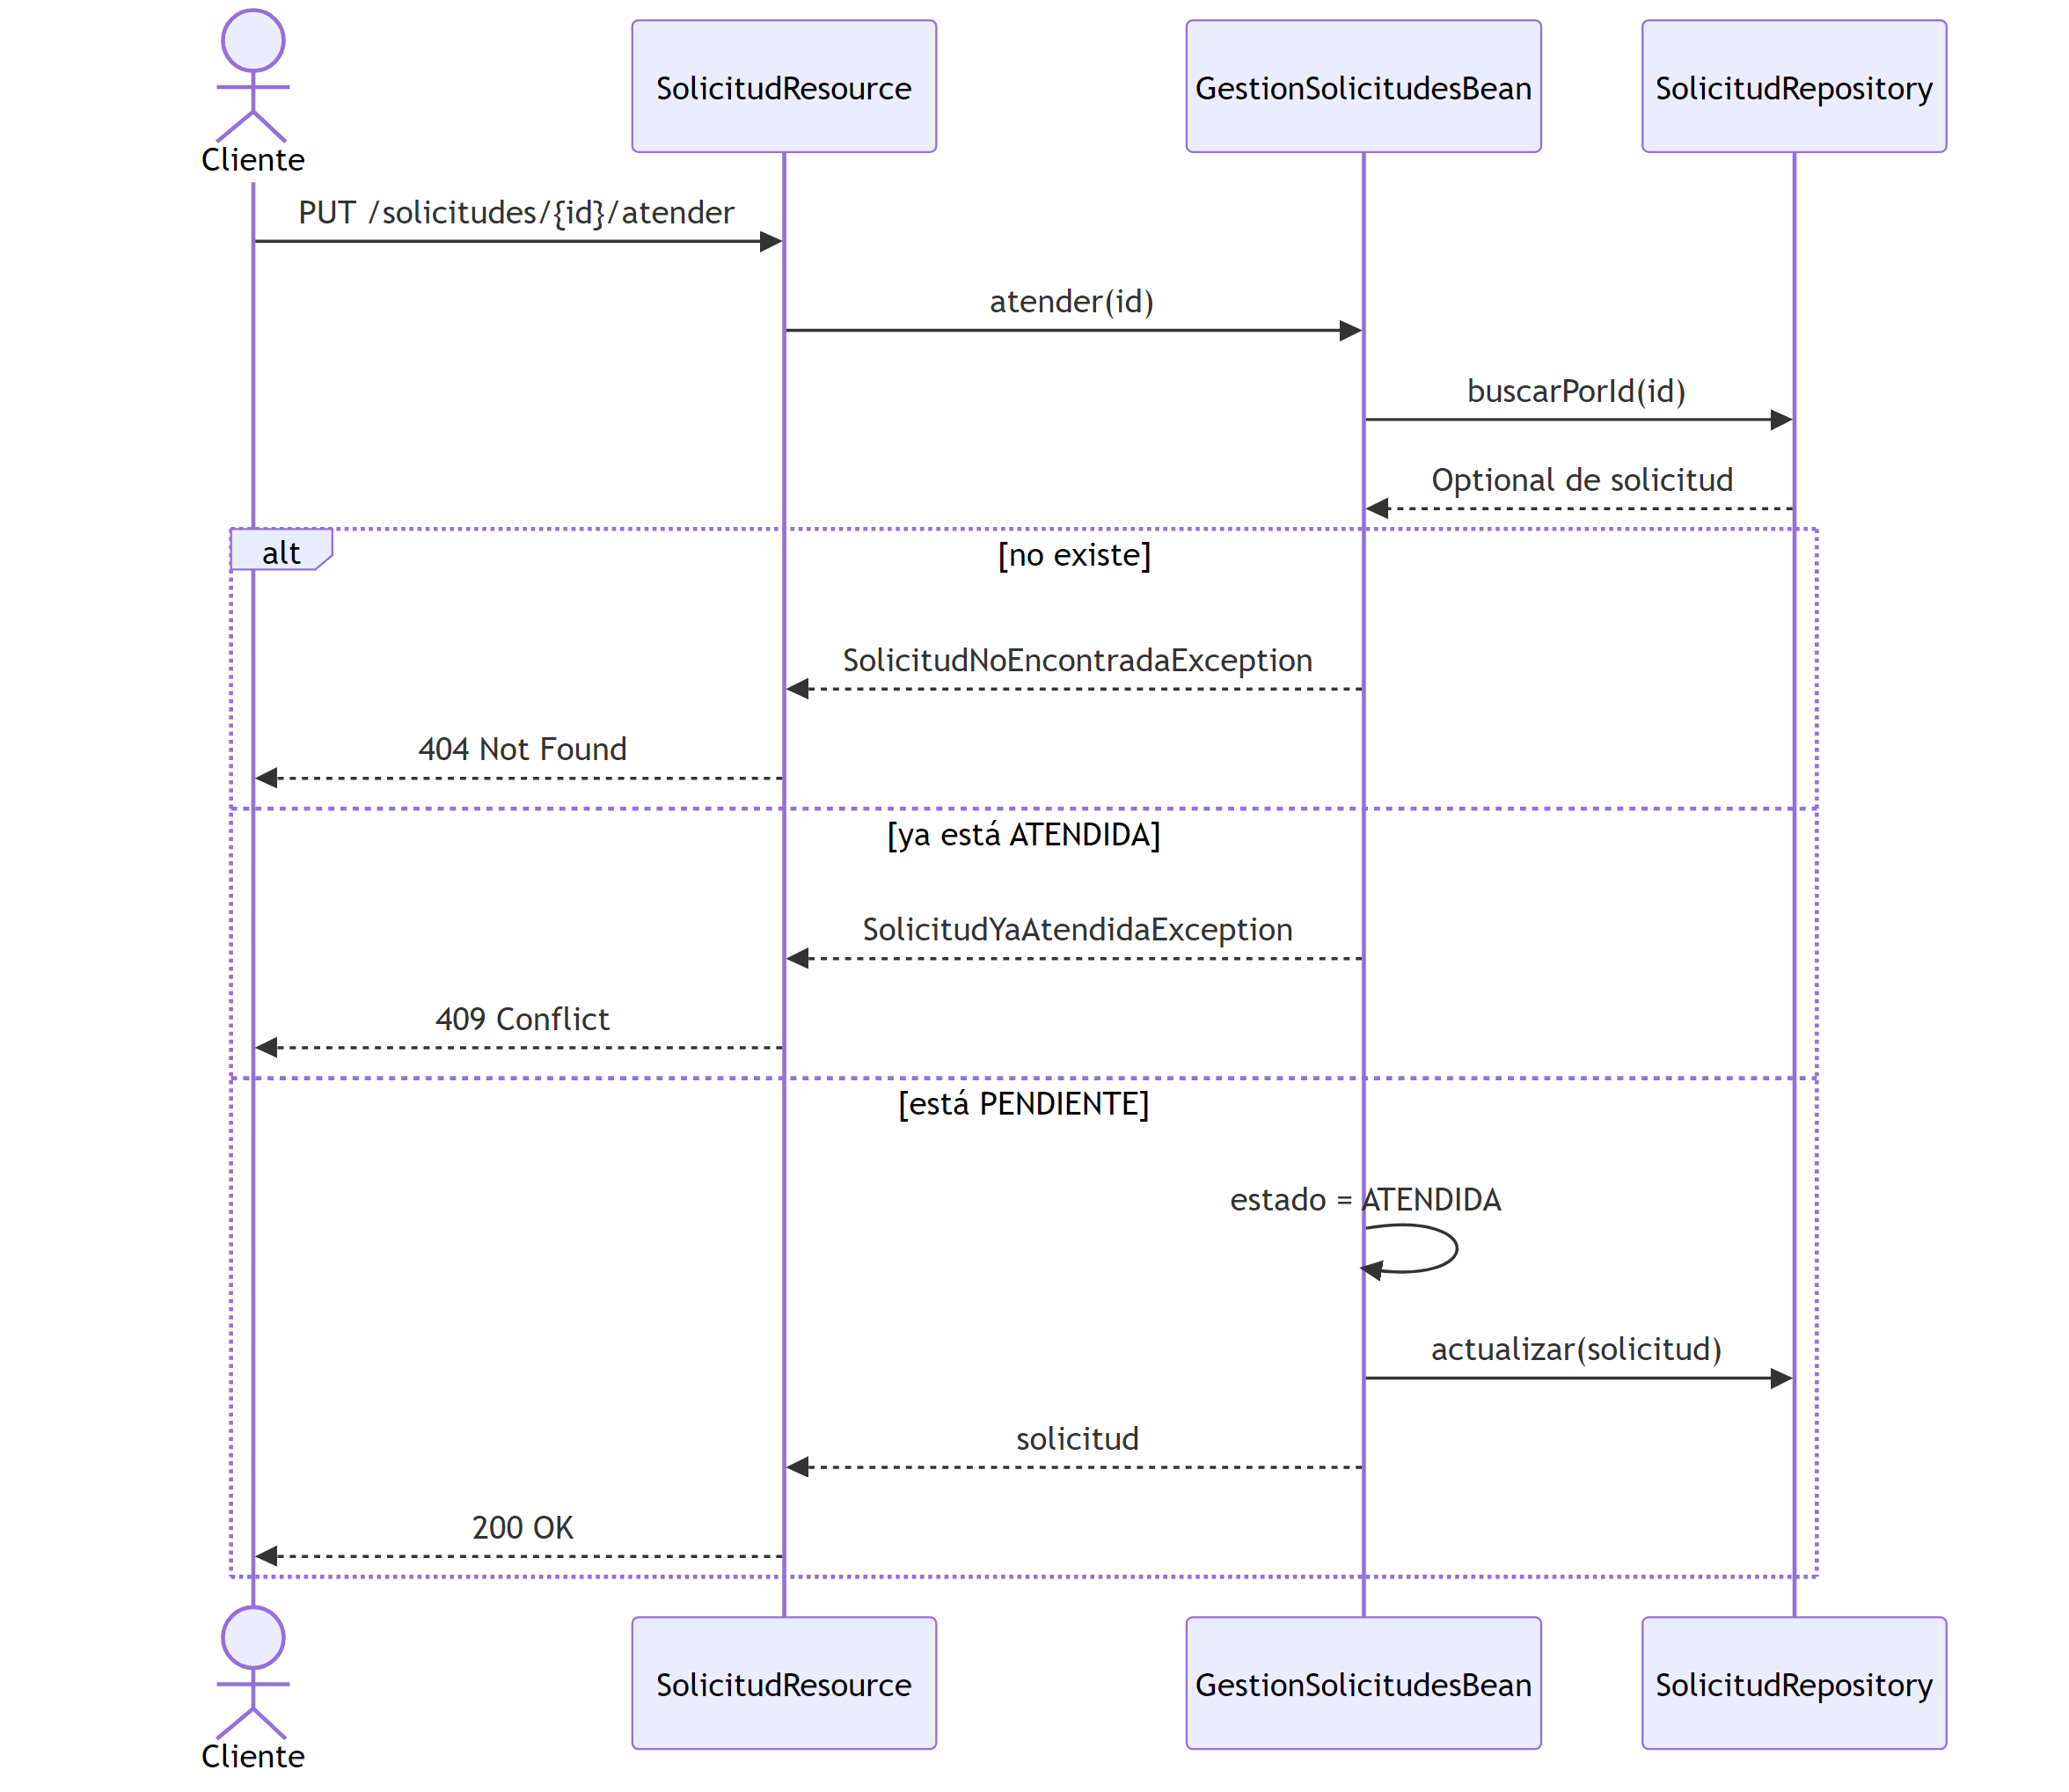
\includegraphics[width=0.8\linewidth]{diagramas/06-secuencia-atender.png}
  \caption{Secuencia: atender una solicitud.}
\end{figure}

\end{document}
